\documentclass[a4paper,12pt]{article}
\usepackage[margin=0.7in]{geometry}
\usepackage{algorithm}
\usepackage{algpseudocode}
\usepackage{tikz}
\usepackage[cm-default]{fontspec}
\usepackage[hidelinks]{hyperref}
\usepackage{xunicode}
\usepackage{xltxtra}
\usepackage{amsfonts, amsmath}
\setlength{\tabcolsep}{0.6em} % for the horizontal padding
{\renewcommand{\arraystretch}{1.5}% for the vertical padding
\algnewcommand{\LineComment}[1]{\State \(\triangleright\) #1}
\usepackage{amsthm}

\usepackage[utf8]{inputenc}
\newtheorem*{theorem}{Θεώρημα}
\newtheorem*{lemma}{Λήμμα}

\usepackage[greek]{babel}
\usepackage{xgreek}
\usepackage{algpseudocode, listings}
\setmainfont{Times New Roman}
\usepackage{titling}
\newcommand{\N}{\ensuremath{\mathbb N} }
\newcommand{\A}{\ensuremath{\mathcal A} }
\newcommand{\pset}[1]{\ensuremath{\mathcal P( #1 )}}
\newcommand{\pr}[1]{\ensuremath{\mathbb P [ #1 ]}}
\newcommand{\ev}[1]{\ensuremath{\mathbb E [ #1 ]}}
\newcommand{\R}{\ensuremath{\mathbb R}}
\newcommand{\opt}{\textsc {Opt}}

\usepackage{graphicx}


\title{ \textbf{Τεχνητή Νοημοσύνη}  \\ 1o Προγραμματιστικό Θέμα \\ Αναφορά Εργασίας \\ \small{Ακ. Έτος 2018-2018}}
\author{\textbf{Μέλη ομάδας (αλφαβητικά)} \\ Εμμανουήλ Παναγιώτου (03115079) -- \texttt{el15079@mail.ntua.gr} \\  Μάριος Παπαχρήστου (03115101) -- \texttt{papachristoumarios@gmail.com} \\ \noindent\rule{0.9\textwidth}{1pt}}
\date{\emph{"It's going to be interesting to see how society deals with artificial intelligence, but it will definitely be cool". --Colin Angle}} 


\begin{document}

\maketitle

\section{Σκοπός Εργασίας} 

Σε αυτή την εργασία υλοποιούμε το βασικό κορμό μιας ευφυούς υπηρεσίας εξυπηρέτησης πελατών ταξί. Συγκεκριμένα,θεωρούμε ότι υπάρχει ένας πελάτης που βρίσκεται σε μια ορισμένη τοποθεσία, ο οποίος διαθέτει κινητό τηλέφωνο με GPS και επιθυμεί να καλέσει ένα ταξί. Η υπηρεσία διαθέτει μια βάση δεδομένων με όλα τα διαθέσιμα ταξί και τη γεωγραφική θέση στην
οποία βρίσκονται κάθε χρονική στιγμή, η οποία θεωρητικά θα πρέπει να ανανεώνεται συνεχώς. Η υπηρεσία θα πρέπει να εντοπίζει και να ειδοποιεί το ταξί που μπορεί να μεταβεί πιο γρήγορα στη θέση του πελάτη ώστε να τον εξυπηρετήσει. Ο χάρτης δίνεται απο δειγματοληπτημένα σημεία οδών από την πόλη της Αθήνας και ο τρόπος εύρεσης της βέλτιστης επιλογής γίνεται με τη χρήση του αλγορίθμου Α*. 

\section{Αντικειμενοστραφής Σχεδιασμός} 

Η παρούσα εργασία αναπτύχθηκε σε γλώσα Java, με γνώμονα τον αντικειμενοστραφή σχεδιασμό. Χρησιμοποιήθηκαν κλάσεις για τα Ταξί (Taxi), τους Πελάτες (Client), τις Κορυφές (Node), τις ακμές (Edge), τους εκτιμητές για τον Α* (Estimator) και τον συνολικό γράφο (Graph). Η κλάση (Point) απλά κρατάει μια γραμμή εισόδου του αρχείου csv. Τέλος χρησιμοποιήθηκε μια κλάση (Visual) για την παραγωγή των αρχείων KML ώστε να γίνεται η απεικόνιση των αποτελεσμάτων στον χάρτη. Για τις δομές δεδομένων χρησιμοποιήθηκαν επίσης κλάσεις των standard βιβλιοθηκών της Java. 

\section{Δημιουργία Γραφήματος}

Η δημιουργία του γράφου γίνεται στον constructor της κλάσης (Graph). Στόχος είναι να παράξουμε μια λίστα από αντικέιμενα (Node). Κάθε Node αντιστοιχεί (μέσω των atributes x, y) σε μια συντεταγμένη και περιέχει μια λίστα απο Edges (adjacent) που αντιστοιχούν στις ακμές του Node. Αρχικά διατρέχουμε το αρχείο csv παράγοντας έτσι αντικείμενα Point. Σε κάθε συντεταγμένη υπάρχει περίπτωση (αν είναι διασταύρωση) να αντιστοιχούν πολλά αντικείμενα Point όμως θέλουμε αυτά να αντιστοιχούν σε ένα μοναδικό Node στον γράφο. Έτσι δημιουργείται η ανάγκη για δύο Hashtables (nodesMap, pointsMap) τα οποία αντιστοιχούν , ένα Node σε πολλά Points και ένα Point σε ένα Node αντίστοιχα. Επίσης για να δημιουργούμε ένα Node για κάθε συντεταγμένη κρατάμε ένα Set από όλα τα Nodes. Έτσι όταν πετύχουμε μια συντεταγμένη πολλές φορές, θα δημιουργηθέι ένα μοναδικό αντικείμενο Node για αυτήν. Έχοντας όσα χρειαζόμαστε, διατρέχουμε την λίστα όλων των Points και για κάθε Point βρίσκουμε το Node στο οποίο αυτό αντιστοιχεί (pointsMap). Έπειτα πηγαίνοντας μια θέση πίσω και μία μπροστά στην λίστα με τα Points, γνωρίζουμε ότι αυτά τα δύο είναι γείτονες του Point στο οποίο βρισκόμαστε. Οπότε ελέγχουμε αν βρίσκονται στην ίδια οδό, βρίσκουμε τα αντίστοιχα previous Node και next Node (πάλι μέσω του pointsMap), φτιάχνουμε αντικείμενα Edge από το Node που βρισκόμαστε στο previous και next, και τις προσθέτουμε στην λίστα adjacent του Node που βρισκόμαστε. Συνεχίζοντας αυτή τη διαδικασία για όλα τα δεδομένα εισόδου, φτιάχνουμε την λίστα από Nodes που χρειαζόμαστε. Κάθε Node μέσω της λίστας adjacent δείχνει στους Nodes γείτονες του. Το μήκος κάθε ακμής $\{u, v\} \in E$ τίθεται ίσο με την γεωγραφική απόσταση σε km δηλαδή 

$$w(u, v) = \mathrm{geo}(u, v) = 111.18957696 \times \arccos \left [ \sin \phi_u \sin \phi_v + \cos \phi_u \cos \phi_v \cos (\theta_u - \theta_v) \right ]$$



\section{Αλγόριθμος Α*}

\subsection{Περιγραφή Αλγορίθμου}
Για την υλοποίηση του Α* χρησιμοποιήθηκαν δύο hashtables για να κρατήσουμε τις $f(v)$ και $g(v)$. Επίσης χρησιμοποιήθηκε ένα HashSet για τη διατήρηση του κλειστού συνόλου και μια ουρά προτεραιότητας \texttt{PriorityQueue<Estimator>} στην οποία τηρούταν το μέτωπο αναζήτησης (ανοικτό σύνολο). Κάθε φορά, από το μέτωπο αναζήτησης αφαιρούνταν ο κόμβος με την ελάχιστη τιμή $$f(v) = g(v) + h(v)$$ όπου $h(v)$ η ευριστική συνάρτηση. Αν ο $v$ ήταν στόχος τότε η αναζήτηση τερμάτιζε. Σε κάθε άλλη περίπτωση ο αλγόριθμος έκανε relax στις κορυφές στις οποίες βελτιώνονταν το $g(v)$. 

\subsection{Ευριστική Συνάρτηση}

Δεδομένης της γεωμετρίας της πόλης, η ευριστική συνάρτηση που διαλέξαμε είναι η Νόρμα Ταξί $L_1$ από τον κοντινότερο στόχο με τύπο 

$$h(v) = \min_{g \in G} h_g(v)$$

όπου $G = \{ g \in V \mid g \text{ στόχος} \}$ με $$h_g(v) = \frac 1 {\sqrt 2} \mathrm{geo}(v, g)$$
 
Για να επιστρέψει σωστά αποτελέσματα ο Α* θα πρέπει η ευριστική συνάρτηση να υποεκτιμά το πραγματικό κόστος $\delta (v \to t)$. 
\subsection{Αποθήκευση Διαδρομών} 

Για να τηρήσουμε τις διαδρομές χρησιμοποιούμε ένα \texttt{Hashtable<Node, Stack<Pair>>} και σε κάθε relaxation προσθέτουμε στη στοίβα την τιμή που βρίσκουμε (η οποία μικραίνει συνεχώς) αφού αφαιρέσουμε πρώτα οποιαδήποτε μεγαλύτερη τιμή. Ο πίνακας κατακερματισμού θα χρησιμεύσει στην εκτύπωση των συντομότερων διαδρομών. Ο κατευθυνόμενος υπολειμματικός γράφος $H$ είναι DAG. Κάνοντας μια αναζήτηση από την κορυφή--στόχο στην αρχή μπορούμε να φτιάξουμε το γράφημα των ισοδύναμων βέλτιστων διαδρομών για τις τιμές των εκτιμήσεων της πραγματικής απόστασης του κάθε κόμβου σε κάθε χρονική στιγμή με τη βέλτιστη (συγκλίνουσα) εκτίμηση. 

\section{Αποτελέσματα}

\subsection{Testcase Άσκησης} 

Ο χάρτης για την αποτίμηση των αποτελεσμάτων βρίσκεται εδώ:
\url{https://drive.google.com/open?id=1YxWv5TfQ8e8Q4oBy8NvlUeZeGtOheg1Z&usp=sharing}

Το αποτέλεσμα για το παράδειγμα βρίσκεται παρακάτω
\begin{figure}[H]
    \centering
    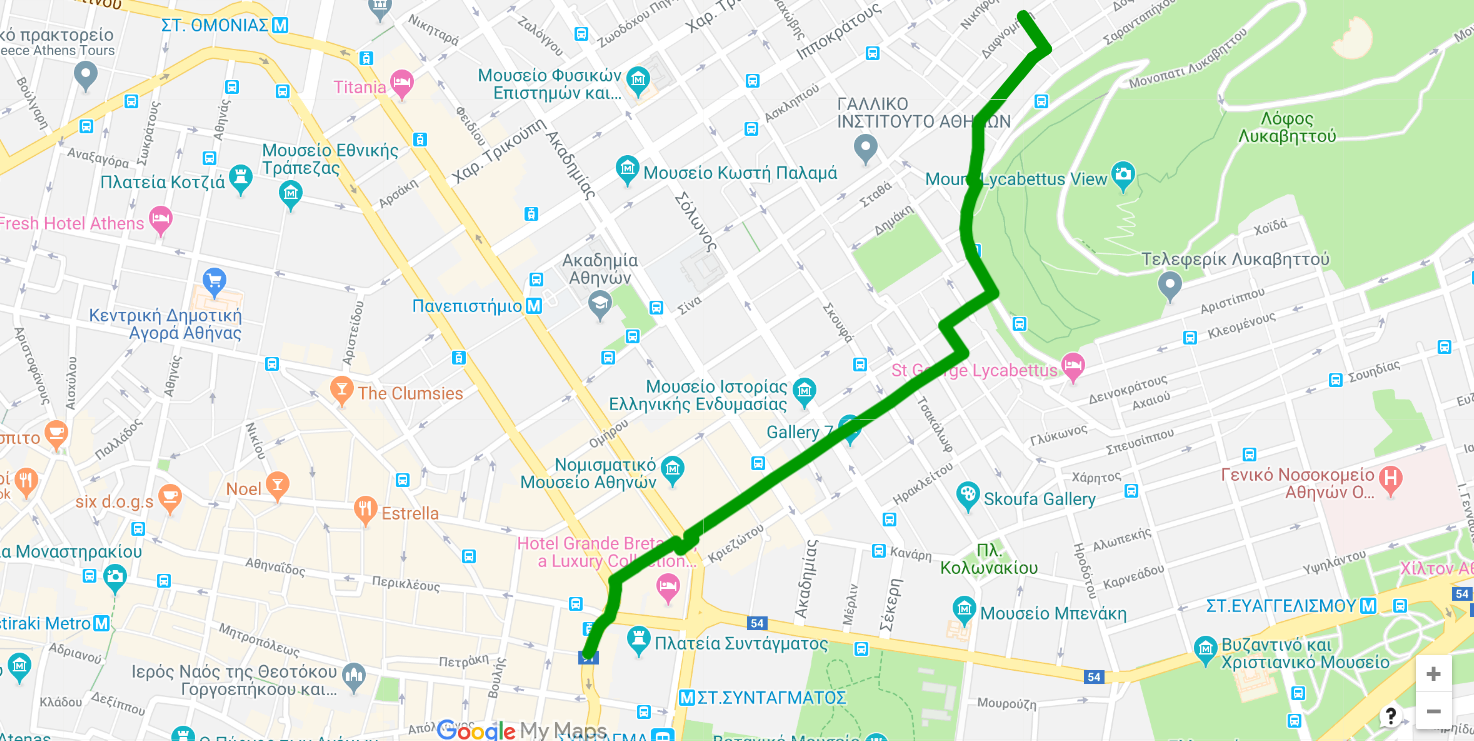
\includegraphics[scale=0.3]{example.png}
    \caption{Αποτέλεσμα για το παράδειγμα από το kml}
    \label{fig:my_label}
\end{figure}

Από το Google Maps αναζητήσαμε την ίδια διαδρομή και λάβαμε το ίδιο αποτέλεσμα

\begin{figure}[H]
    \centering
    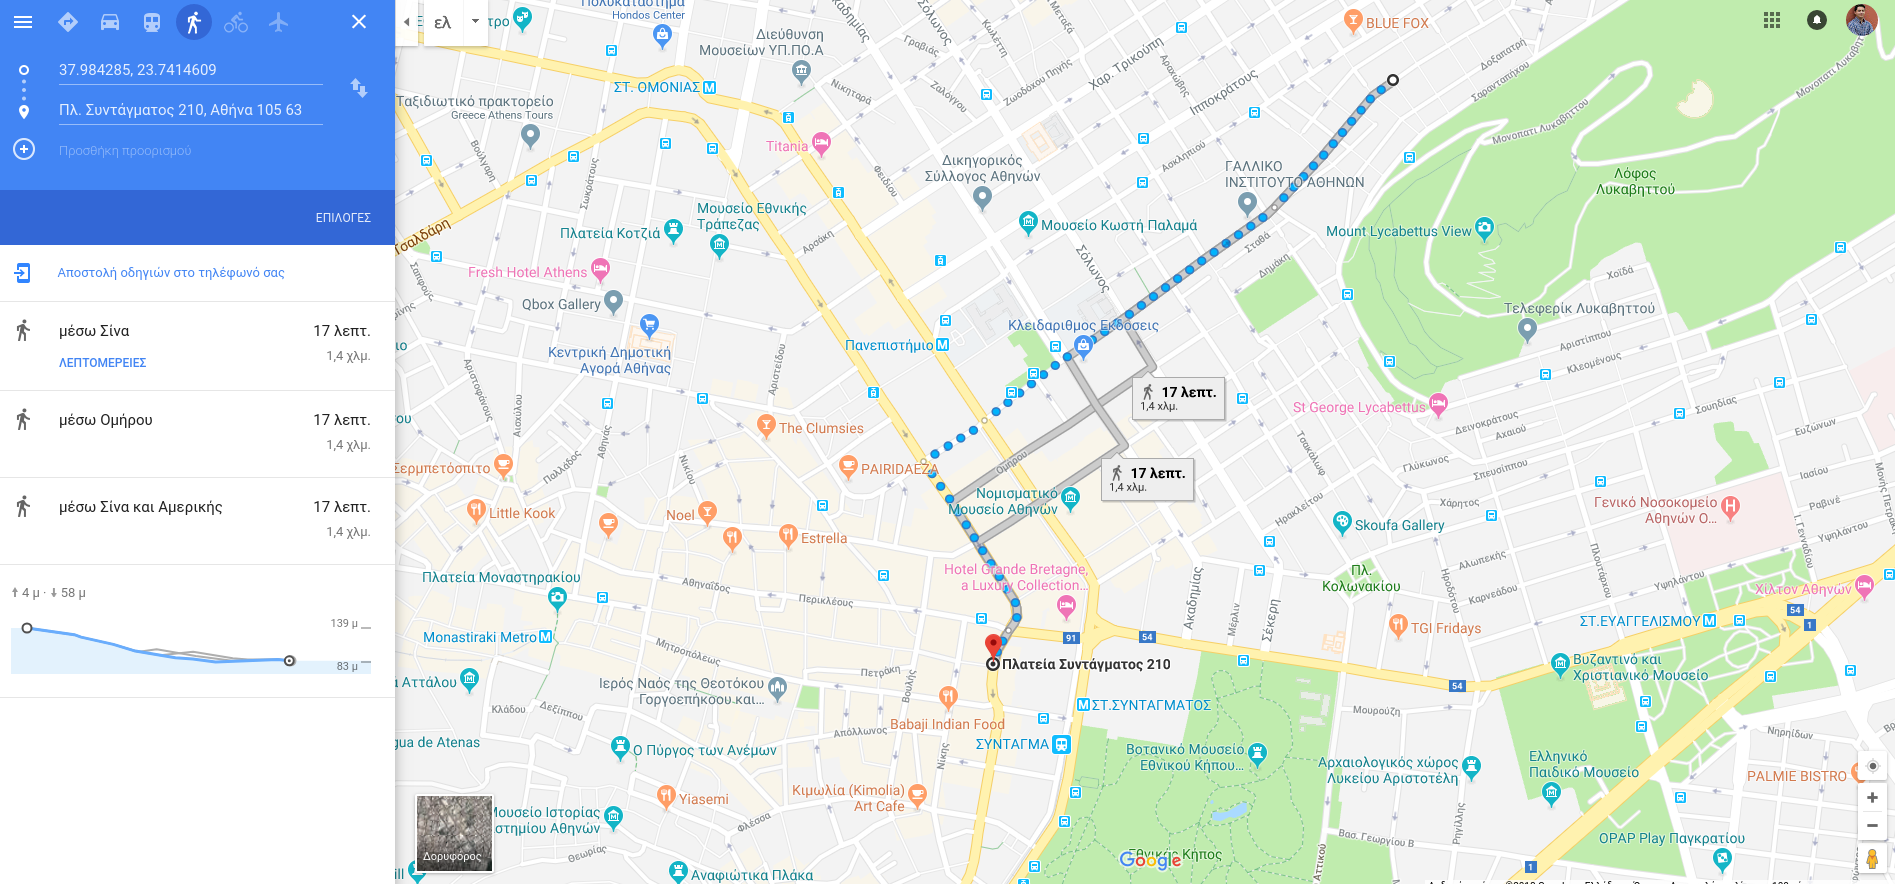
\includegraphics[scale=0.25]{correct.png}
    \caption{Αποτέλεσμα για το παράδειγμα από Google Maps}
    \label{fig:my_label}
\end{figure}

Τα μήκη και των δύο διαδρομών είναι 1.385 km όπως και στην διαδρομή που προτείνει το Google Maps. Το kml αρχείο βρίσκεται στο \texttt{original.kml}.


\subsection{Επιπλέον Testcases}

Για τις ανάγκες της άσκησης, δημιουργήσαμε επιπλέον testcases. 

\paragraph{Αξιολόγηση Ευριστικής -- Δύο Στόχοι} Στο πρώτο testcase δημιουργήσαμε δύο στόχους οι οποίοι ισαπέχουν από τον πελάτι (κίτρινο χρώμα) και ο πελάτης φαίνεται με μωβ. Τα ταξί απέχουν 0.409 km από τον πελάτη

\begin{figure}[htp]
\centering
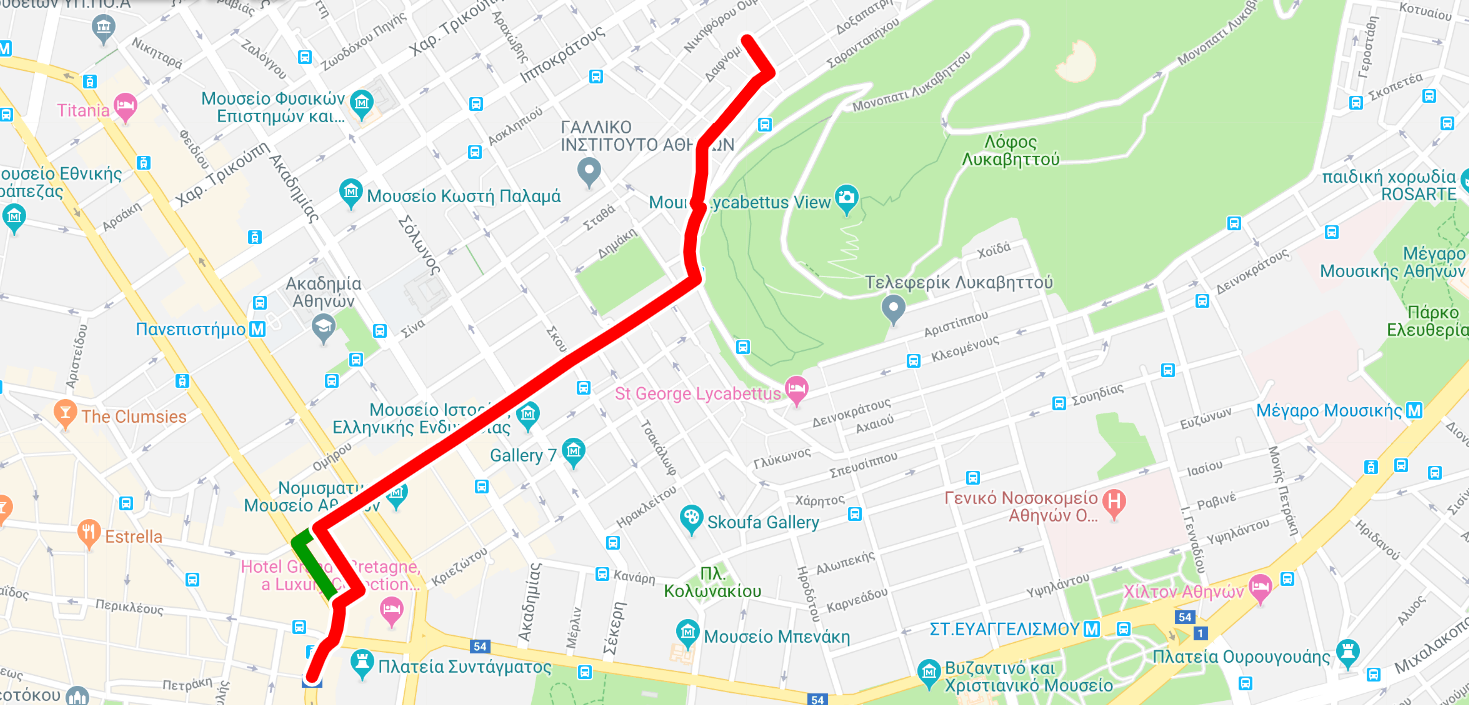
\includegraphics[scale=0.3]{second.png}
\caption{Αξιολόγηση Ευριστικής Συνάρτησης}
\label{}
\end{figure}  


\begin{thebibliography}{9}

\bibitem{norvig} Russell, Stuart J., and Peter Norvig. Artificial intelligence: a modern approach. Malaysia; Pearson Education Limited,, 2016.

\bibitem{stamou} Στάμου Γ., Τεχνητή Νοημοσύνη, Διαφάνειες

\end{thebibliography}

\end{document}
